\chapter{Trabalhos Correlatos}

\noindent Este capítulo aborda os trabalhos que são correlatos a esta pesquisa, bem como descreve como estes trabalhos diferem do realizado
por esta pesquisa.
\clearpage

\section{Ferramentas de ETL}



\subsection{ARKTOS II}
ARKTOS II: modela os processos de ETL

\subsection{PygramETL}
PygramETL: 

\subsection{ETLMR}
ETLMR é um framework de ETL que utiliza \textit{MapReduce} para atingir escalabilidade. Ele suporta esquemas de DW como o esquema estrela, o \textit{snowflake}, e o \textit{slowly changing dimensions} \cite{liu:2011}. 

A figura \ref{etlmr} 

\begin{figure}[h]
	\centering
	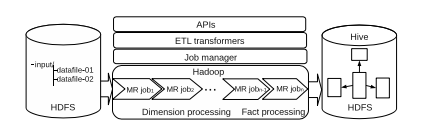
\includegraphics[scale=0.7]{fig/cloudetl.png}
	\caption{Fluxo de dados ETL no framework MapReduce (Adaptado de \cite{liu:2011})}
	\label{etlmr}
\end{figure}


\subsection{CloudETL}

O framework CloudETL é uma solução para processos de ETL que usa \textit{Hadoop} para paralelizar fluxos de ETL e \textit{Hive} para processar os dados de forma distribuída. Para o CloudETL o \textit{Hadoop} é a plataforma de execução dos processos de ETL e o \textit{Hive} é o sistema de armazenamento. Conforme a figura \ref{cloudetl}, os componentes do CloudETL são as APIs (interfaces de programação de aplicação), um conjunto de elementos para efetuar as transformações nos dados identificados como ETL \textit{transformers}, e um gerenciador de tarefas que controla a execução das tarefas submetidas ao \textit{Hadoop}. 

CloudETL fornece suporte de alto nível em ETL para construção de diferentes esquemas de DW, como esquema estrela, \textit{snowflake} e SCD (\textit{slowly changing dimensions}). Ele facilita a implementação de processos de ETL em paralelo e aumenta a produtividade do programador significativamente. Esta abordagem facilita as atualizações de SCDs em um ambiente distribuído \cite{liu:2013}.

\begin{figure}[h]
	\centering
	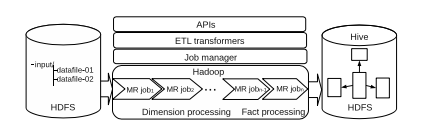
\includegraphics[scale=0.7]{fig/cloudetl.png}
	\caption{Arquitetura do CloudETL (Adaptado de \cite{liu:2013})}
	\label{cloudetl}
\end{figure}

O CloudETL é uma alternativa quando o problema é o processamento de um grande volume de dados por possuir a propriedade de processamento distribuído, porém não oferece nenhum suporte para modelagem de processos de ETL ficando a cargo do programador ou da equipe responsável pelo projeto de DW. 


\subsection{P-ETL}
P-ETL:

\subsection{Big-ETL}
Big-ETL: Foca na paralelização e distribuição.

\subsection{FramETL}
FramETL

\subsection{Pentaho}
Pentaho

\subsection{Talend Studio}
Talend Studio for Data Integration

\subsection{CloverETL}
CloverETL

\subsection{Oracle Data Integrator (ODI)}
Oracle Data Integrator (ODI)